% !TeX spellcheck = cs_CZ
%{\tikzset{external/prefix={tikz/FYZII/}}
% \tikzset{external/figure name/.add={ch20_}{}}
%---------------------------------------------------------------------------------------------------
% file fey2ch20.tex
%---------------------------------------------------------------------------------------------------
%=========================== Kapitola: Řešení Maxwellových rovnic ve volném prostoru  ==============
\setchaptertoc
\chapter{Řešení Maxwellových rovnic ve volném prostoru}\label{fyz:IIchapXX}

  \section{Vlny ve volném prostoru. Rovinné vlny}\label{fyz:IIchapXXsecI}
  \section{Trojrozměrné vlny}\label{fyz:IIchapXXsecII}
  \section{Vědecká obrazotvornost}\label{fyz:IIchapXXsecIII}
  \section{Kulové vlny}\label{fyz:IIchapXXsecIV}
  \section{Příklady a cvičení}\label{fyz:IIchapXXsecV}


    \begin{figure}[ht!] %\ref{fyz:fig643}
      \centering
      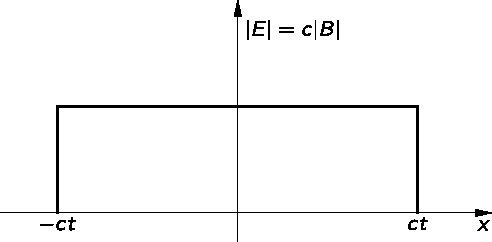
\includegraphics[width=0.7\linewidth]{fyz_fig643.pdf}
      \caption{
               (\cite[s.~707]{Feynman02})}
      \label{fyz:fig643}
    \end{figure}


    \begin{figure}[ht!] %\ref{fyz:fig644}
      \centering
      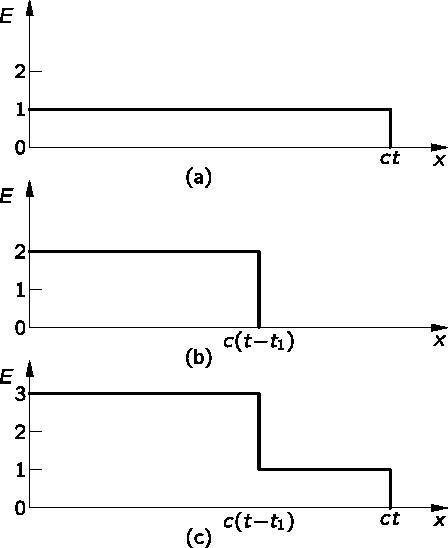
\includegraphics[width=0.7\linewidth]{fyz_fig644.pdf}
      \caption{
               (\cite[s.~707]{Feynman02})}
      \label{fyz:fig644}
    \end{figure}


    \begin{figure}[ht!] %\ref{fyz:fig645}
      \centering
      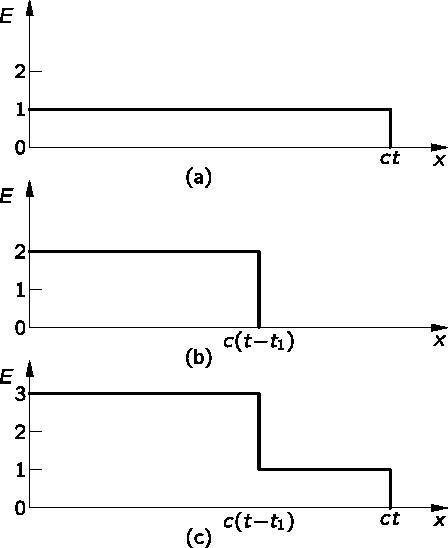
\includegraphics[width=0.7\linewidth]{fyz_fig645.pdf}
      \caption{
               (\cite[s.~707]{Feynman02})}
      \label{fyz:fig645}
    \end{figure}

    \begin{figure}[ht!] %\ref{fyz:fig646}
      \centering
      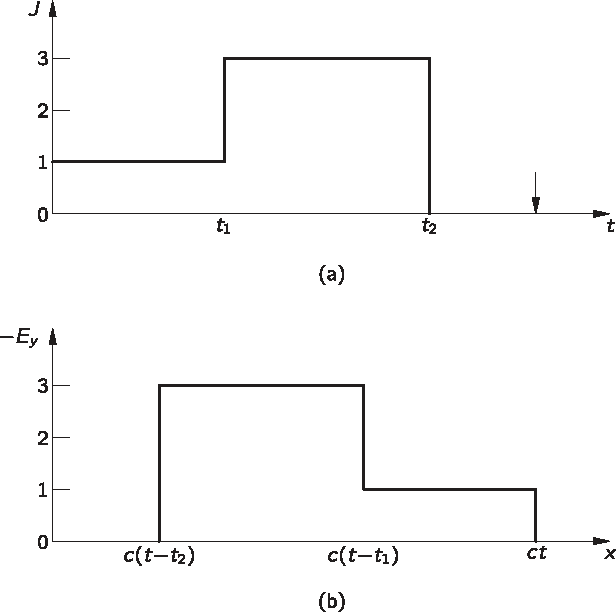
\includegraphics[width=0.7\linewidth]{fyz_fig646.pdf}
      \caption{
               (\cite[s.~707]{Feynman02})}
      \label{fyz:fig646}
    \end{figure}


    \begin{figure}[ht!] %\ref{fyz:fig647}
      \centering
      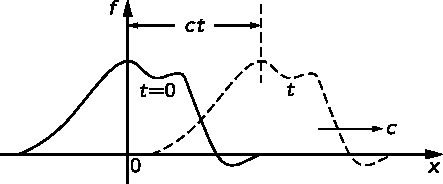
\includegraphics[width=0.7\linewidth]{fyz_fig647.pdf}
      \caption{
               (\cite[s.~707]{Feynman02})}
      \label{fyz:fig647}
    \end{figure}

    \begin{figure}[ht!]
      \centering
      \subcaptionbox{\label{fyz:fig649a}}{\luafigure[0.8]{fyz_fig649a.pdf}}               \newline
      \subcaptionbox{\label{fyz:fig649b}}{\luafigure[0.8]{fyz_fig649b.pdf}}
      \label{fyz:fig649}
      \caption{
               (\cite[s.~748]{Feynman02})}
    \end{figure}
    
    \todo[inline]{Kapitola fey2ch20 je nedodělaná, obsahuje pouze obrázky}
%} %tikzset
%---------------------------------------------------------------------------------------------------